%%%%%%%%%%%%%%%%%%%% author.tex %%%%%%%%%%%%%%%%%%%%%%%%%%%%%%%%%%%
%
% sample root file for your "contribution" to a proceedings volume
%
% Use this file as a template for your own input.
%
%%%%%%%%%%%%%%%% Springer %%%%%%%%%%%%%%%%%%%%%%%%%%%%%%%%%%


\documentclass{svproc}
%
% RECOMMENDED %%%%%%%%%%%%%%%%%%%%%%%%%%%%%%%%%%%%%%%%%%%%%%%%%%%
%

% to typeset URLs, URIs, and DOIs
\usepackage{url}
\usepackage[utf8]{inputenc}
\usepackage{graphicx}
\def\UrlFont{\rmfamily}

\begin{document}
\mainmatter              % start of a contribution
%
\title{Person following robot behavior using Deep Learning}
%
%
\author{Ignacio Condés\inst{1} \and José María Cañas\inst{2}}
%

%
\institute{Universidad Rey Juan Carlos,
	\email{ignacio.condes.m@gmail.com},
	\and
Universidad Rey Juan Carlos, \email{jmplaza@gsyc.es}}

\maketitle              % typeset the title of the contribution

\begin{abstract}
The proposed following behavior combines a \emph{perception} and a \emph{control} module. Perception module addresses the person detection on images using a pretrained TensorFlow SSD \emph{Convolutional Neural Network}. It provides \emph{robustness} over traditional methods, although care has to be put on not losing real-time operation. A \emph{person tracker filter} has been included to alleviate the effect of false positives/negatives. It also extracts faces, which are also analyzed by a \emph{FaceNet} CNN to reidentify the tracked individual. This perception module tells which person in the image has to be followed, even on poorly lightened scenarios. It is combined with depth readings to obtain the relative position of the person. The control module implements a case-based \emph{PID} controller for a reactive smooth response, moving the robot towards the target person. The entire system has been experimentally validated\footnote{\url{https://jderobot.org/Naxvm-tfg}} on a real Turtlebot2 robot, with an Asus Xtion RGBD camera.
% We would like to encourage you to list your keywords within
% the abstract section using the \keywords{...} command.
\keywords{Computer Vision, neural networks, deep learning, robotic behavior}
\end{abstract}
%

%  ---- Intro ----
\section{Introduction}
%
In this project, we aim to establish a scope which covers two fields: \emph{robotics} and \emph{deep learning}.\\

In the last decades, robots have become a powerful allied to humans, as they are leveraged to perform all kind of tasks (hazardous explorations, personal assistance, cleaning, driving, \dots). However, we aim to design them to perform these tasks on the most autonomous way possible, which means not requiring to be controlled on every action (with exceptions, such as surgeon robots). This requires to provide robots a certain intelligence and capabilities to correctly trigger the most suitable action for each possible input stimulus. For this purpose, we can find multiple approaches for different problems (navigation, conversation, \dots).\\

Concretely, this article is dovetailed with \emph{Computer Vision}, which involves connecting cameras to a robot, and taking advantage of this on an autonomous way. Concretely, we will tackle the \emph{person following} challenge, which is based on a behavior governed by a person \emph{detection} system. Many approaches are already existing, such as color filters \cite{rocapal}, or disparities filtering. However, promising \emph{Deep Learning} techniques excel on their image processing variant, as they offer high quality results, accompanied by \emph{robustness} facing lighting issues (Fig. \ref{fig:intro_harsh_light}). This is the set of techniques we have used on this project, so we will describe the basis firstly.\\

\begin{figure}[h]
	\centering
	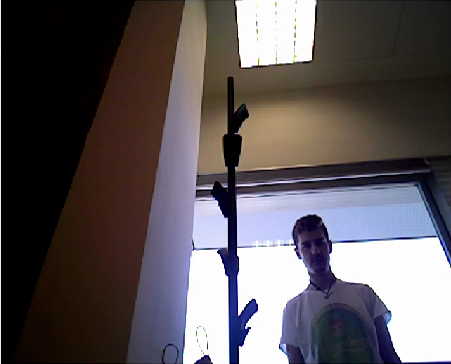
\includegraphics[width=2in]{images/light_ko_2}
	\caption{Harsh lighting situation for \emph{Computer Vision} algorithms.}
	\label{fig:intro_harsh_light}
\end{figure}


In the image detection quandary, the main objective is to determine \emph{presence and position} of a certain object in a given image. For this, we make use on this article of \emph{deep learning} techniques, concretely \emph{Convolutional Neural Networks} (CNNs).\\


This investigation has focused on exploring the synergies existing the two explained fields, making use of \emph{deep learning} to automatically command a robot to follow a determined person. This is achieved making use of two different modules: a \emph{perception} one, focused on the computer vision/deep learning tasks, and an \emph{actuation} module, which implements a case-based behavior, depending on what the perceptive part senses and computes. The designed system has been experimentally validated, as it will be seen on section \ref{sec:experiments}

% ---- Infrastructure ----
\section{Infrastructure}

On this article, we rely on a certain set of hardware/software elements:

\subsection*{Hardware}

\begin{itemize}
	\item \emph{Asus Xtion Pro Live}: RGBD (RGB + Depth) sensor. It counts with a regular digital camera, and with an infrared emitter, which radiates IR beams. Their reflections are retrieved by a depth sensor, which generates a \emph{point cloud} with the measured distance to each reflection surface. A \emph{registration} process is performed in the driver, to project these points into the RGB pixels (due to the spacial offset between both sensors).\\
	
	\item \emph{Turtlebot 2}: 2-wheeled robot, designed for didactic purposes. It counts with 2 freedom degrees on its motors: \emph{angular} movements and \emph{linear} movements.\\
\end{itemize}

\subsection*{Software}

\begin{itemize}
	\item \emph{ROS}: robotics software development framework. It provides, among others, the low level drivers to get correctly communicated with the hardware devices.\\
	
	\item \emph{JdeRobot}: research and educational robotics framework. The taken benefit from this framework is the higher level interfaces to communicate our developed program with the drivers created by ROS.\\
	
	
	\item \emph{TensorFlow}: \emph{deep learning} library recently developed by Google, and already widely adopted by big companies. It operates with \emph{tensors}\footnote{Generic data structure with a specific number of dimensions.} on an optimized low-level way. It allows GPU parallelization of the operations, which leads to a very efficient implementation of \emph{deep learning} algorithms.\\
	
	
	\item \emph{Python}: high-level interpreted programming language. It is widely used on \emph{machine learning} purposes due to its focus on easiness and \emph{Object Orientation}. It counts with implementations of the previously described libraries and frameworks.\\
\end{itemize}

% ---- Perception module ----
\section{Perception Module}

This is the first component of the developed system. As it name indicates, it is responsible for apprehend the incoming images from the sensor (RGB and depth) images, and generate a significant output to be interpreted by the actuation module. Its structure follows a certain pipeline along the images, which will be analyzed next.


\subsection{Object Detection}

On first place, the incoming RGB images are passed through an \emph{object detection} module. This module is powered by a CNN, which has a special architecture designed for this purpose: SSD (\emph{Single-Shot Multibox Detector}). This kind of detection technique stands out by its prediction speed, because \emph{it performs a single feed-forward pass} of the image through the network, unlike the rest of \emph{state-of-the-art} techniques (which are consequently much slower, AS CAN BE SEEN ON [tabla experimentos object detector]).\\


IMAGEN ESTRUCTURA RED (5.6 tfg)
This neural architecture is formed putting together a succession of blocks:

\begin{enumerate}
	\item \emph{Preprocessing:} as this kind of neural networks work with a fixed image shape (300$\times$300 px in this case, the most typical one among other SSD implementations).\\
	
	\item \emph{Feature Extraction:} a first group of layers (\emph{base network}) deals the \emph{feature extraction} part. As it is composed by a concatenation of \emph{convolutional} layers, the resulting activation maps are gradually smaller and deeper. So, 6 intermediate sets, composed by activation maps of a certain depth are extracted from this concatenation, with progressive sizes (suitable for different objects shapes). This way, we obtain the 6 activation maps reflected on the Table TABLA PAG 55 TFG.
	
	\item \emph{Box Prediction:} later, on a parallel way for each set, the activation maps are traversed, generating \emph{prior} boxes on each point of them, with different aspect ratios. These \emph{priors} are convolved with small filters, which output \emph{adjustments} for each box, and \emph{softmaxed} confidences for each of the classes that the network knows. IMAGEN PERRO GATO
	
	\item \emph{Postprocessing:} it combines the detections of each of the 6 sets, only retaining the most confident detections (\emph{Non-Maximum Supression}), and adjusting and scaling the obtained bounding boxes to the original image shape. 
\end{enumerate}

This system provides an accurate and efficient object detection, returning for each processed image:

\begin{itemize}
	\item \emph{Classes:} the detected classes (person, cell phone, airplane, dog \dots) inferred for each detected object.
	
	\item \emph{Scores:} the confidence $\in [0,1]$ the network has on each object belonging to the decided class.
	
	\item \emph{Boxes:} the coordinates of the rectangular \emph{bounding box} which wraps the detected object, expressed as the coordinates of two opposite corners of it.
\end{itemize}

However, our system only retains those detection corresponding to \emph{persons}, as it is what we are interested to follow.\\


Hence, this results on a light \emph{person detection}, perfectly capable to work on a real-time operation on a standard level hardware. Our implementation is capable to handle different network models and architectures on a \emph{plug and play} model, just with the model file (in the specific TensorFlow \texttt{.pb} format).



\subsection{Face detection}

Once we have detected the existing persons on the image, we will look for their faces, in order to know whether any of them corresponds to the person to follow. To do so, we will perform \emph{face reidentification}, which needs in first place to detect each person face. To do so, we implement the classical Viola and Jones [31 tfg] face detection algorithm. This algorithm, which comprises \emph{Haar} features (Fig. --), is a simple algebraic method which takes advantage of the typical illumination pattern of a face (due to its physical shape) to detect promising regions of the input image to contain a face. This image is divided into \emph{regions}, which are passed through a \emph{cascade} of tests, where the non-compliant regions are immediately discarded. The accepted ones pass to a slightly more complex feature each time, and the regions which pass all the features are supposed to contain a face. This progressive region dismiss makes it an efficient algorithm, capable of run simultaneously with the rest of processes. This entire process is performed with an OpenCV\footnote{Open source image processing library.} method.\\

As we already knew where the detected persons are in the image, this face detection process is only performed inside the persons bounding boxes.



\subsection{Face reidentification (\emph{FaceNet})}

If it is achieved to find 




















% ---- Bibliography ----
%
\begin{thebibliography}{6}
%

\bibitem {smit:wat}
Smith, T.F., Waterman, M.S.: Identification of common molecular subsequences.
J. Mol. Biol. 147, 195?197 (1981). \url{doi:10.1016/0022-2836(81)90087-5}

\bibitem {may:ehr:stein}
May, P., Ehrlich, H.-C., Steinke, T.: ZIB structure prediction pipeline:
composing a complex biological workflow through web services.
In: Nagel, W.E., Walter, W.V., Lehner, W. (eds.) Euro-Par 2006.
LNCS, vol. 4128, pp. 1148?1158. Springer, Heidelberg (2006).
\url{doi:10.1007/11823285_121}

\bibitem {fost:kes}
Foster, I., Kesselman, C.: The Grid: Blueprint for a New Computing Infrastructure.
Morgan Kaufmann, San Francisco (1999)

\bibitem {czaj:fitz}
Czajkowski, K., Fitzgerald, S., Foster, I., Kesselman, C.: Grid information services
for distributed resource sharing. In: 10th IEEE International Symposium
on High Performance Distributed Computing, pp. 181?184. IEEE Press, New York (2001).
\url{doi: 10.1109/HPDC.2001.945188}

\bibitem {fo:kes:nic:tue}
Foster, I., Kesselman, C., Nick, J., Tuecke, S.: The physiology of the grid: an open grid services architecture for distributed systems integration. Technical report, Global Grid
Forum (2002)

\bibitem {onlyurl}
National Center for Biotechnology Information. \url{http://www.ncbi.nlm.nih.gov}


\end{thebibliography}
\end{document}
